\documentclass{article}
\usepackage[margin=1in]{geometry}
\usepackage{amsmath,amsthm,amssymb}
\usepackage{bbm,enumerate,mathtools}
\usepackage{tikz,pgfplots}
\usepackage{chessboard}
\usepackage[hidelinks]{hyperref}
\usepackage{multicol} % Problem 35

\newenvironment{question}{\begin{trivlist}\item[\textbf{Question.}]}{\end{trivlist}}
\newenvironment{note}{\begin{trivlist}\item[\textbf{Note.}]}{\end{trivlist}}
\newenvironment{references}{\begin{trivlist}\item[\textbf{References.}]}{\end{trivlist}}
\newenvironment{related}{\begin{trivlist}\item[\textbf{Related.}]\end{trivlist}\begin{enumerate}}{\end{enumerate}}


\begin{document}
\rating{1}{2}
The number of ways to draw a triangle on a triangular grid is given by \[
  \sum_{k=1}^{n-1} k\cdot t(n-k) = \binom{n+2}{4}
\] where $t(m)$ is the $m$-th triangular number.
\\~\\
The number of ways to draw a square on a square grid is given by \[
  \sum_{k=1}^{n-1} k\cdot (n-k)^2 = n^2\left(\frac{n^2 - 1}{12}\right)
\] the 4-dimensional pyramidal number.
\\~\\
The number of ways to draw a hexagon on a hexagonal grid is given by \[
  \sum_{k=1}^{n-1} k\cdot h(n-k) = \sum_{k=1}^{n-1} k^3 = t(n-1)^2
\] where $h(m)$ is the $m$-th hexagonal number.
\begin{figure}[ht!]
  \centering
  % Triangle
  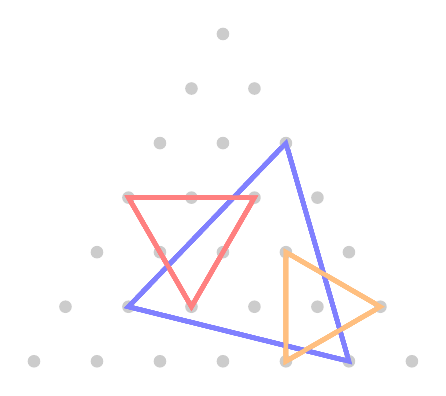
\begin{tikzpicture}[scale=0.8]
    \foreach \x in {1,...,7} {
      \foreach \y in {1,...,\x} {
        \fill[gray!40] ({\x - \y/2}, {sqrt(3)/2 * \y}) circle (0.1);
      }
      \draw[ultra thick, blue!50] (2, {sqrt(3)})--(4.5, {5/2*sqrt(3)})--(5.5, {sqrt(3)/2})--cycle;
      \draw[ultra thick, red!50] (3, {sqrt(3)})--(4, {4/2*sqrt(3)})--(2, {4/2*sqrt(3)})--cycle;
      \draw[ultra thick, orange!50] (4.5, {sqrt(3)/2})--(4.5, {3/2*sqrt(3)})--(6, {sqrt(3)})--cycle;
    }
  \end{tikzpicture}
  % Hexagon
  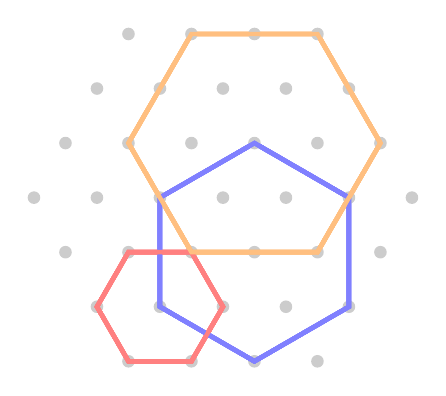
\begin{tikzpicture}[scale=0.8]
    \foreach \y/\n/\k in {1/4/0, 2/5/0, 3/6/0, 4/7/0, 5/6/1, 6/5/2, 7/4/3} {
      \foreach \x in {1,...,\n} {
        \fill[gray!40] ({\x - \y/2 + \k}, {sqrt(3)/2 * \y}) circle (0.1);
      }
      \draw[ultra thick, blue!50] (2.5, {sqrt(3)/2 * 1})--(1, {sqrt(3)/2 * 2})--(1, {sqrt(3)/2 * 4})--(2.5, {sqrt(3)/2 * 5})--(4, {sqrt(3)/2 * 4})--(4, {sqrt(3)/2 * 2})--cycle;
      \draw[ultra thick, red!50] (0.5, {sqrt(3)/2 * 1})--(0, {sqrt(3)/2 * 2})--(0.5, {sqrt(3)/2 * 3})--(1.5, {sqrt(3)/2 * 3})--(2, {sqrt(3)/2 * 2})--(1.5, {sqrt(3)/2 * 1})--cycle;
      \draw[ultra thick, orange!50] (1.5, {sqrt(3)/2 * 7})--(3.5, {sqrt(3)/2 * 7})--(4.5, {sqrt(3)/2 * 5})--(3.5, {sqrt(3)/2 * 3})--(1.5, {sqrt(3)/2 * 3})--(0.5, {sqrt(3)/2 * 5})--cycle;
    }
  \end{tikzpicture}
  \hspace{0.7cm}
  % Square
  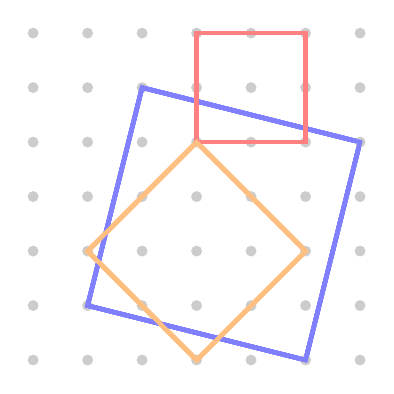
\begin{tikzpicture}[scale=0.692]
    \foreach \x in {1,...,7} {
      \foreach \y in {1,...,7} {
        \fill[gray!40] (\x, \y) circle (0.1);
      }

      \draw[ultra thick, blue!50] (6,1)--(7,5)--(3,6)--(2,2)--cycle;
      \draw[ultra thick, red!50] (4,5)--(6,5)--(6,7)--(4,7)--cycle;
      \draw[ultra thick, orange!50] (2,3)--(4,5)--(6,3)--(4,1)--cycle;
    }
  \end{tikzpicture}
  \caption{
    All connected configurations of $4$ coins. Six out of the seven possible
    polyhexes are present.
  }
\end{figure}
\begin{question}
  Is there a combinatorial explanation for why these numbers have nice closed
  forms?
\end{question}

\begin{related}
  \item Can this be generalized to arbitrary regular $n$-gons in hyperbolic
    space?
  \item How many triangles are on the ``centered triangular number'' grid?

\end{related}
\begin{references}
  \item Problem 25.
  \item \url{https://en.wikipedia.org/wiki/Order-4_pentagonal_tiling}
\end{references}
\end{document}
